\chapter{The Prompt Engineering Ontology: Conceptualization and Encoding}
\label{chapter:4_implementation}
This chapter describes the implementation of PEO by following the approach described by the LOT methodology. 
In the section \ref{section:4_1_conceptualization} we discuss the conceptualization of PEO, in the section \ref{section:4_2_reuse} we discuss the reuse of existing design patterns and in the section \ref{section:4_3_encoding} we describe the encoding process. 
\begin{figure}[H]
    \centering
    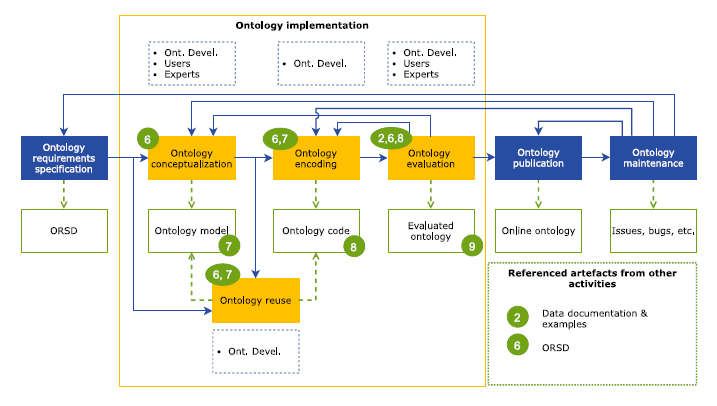
\includegraphics[width=0.9\linewidth]{Figures/fig_14.png}
    \caption{Ontology implementation workflow}
    \label{fig:14}
\end{figure}
Fig. \ref{fig:14} represents the ontology implementation workflow according to LOT.
At the end of this phase, the output is an ontology ready to be published and to be made available online.

\section{Conceptualization}
\label{section:4_1_conceptualization}
The first step in the ontology implementation is the ontology conceptualization, we define of all main concepts in the ontology with the relations among them.
We used \href{draw.io}{https://app.diagrams.net/} software: a free easy-to-use diagramming tool that allows to represent UML diagrams and many more. 
We chose this software over other diagramming tools because it is intuitive, easy to use, and frequently updated moreover with draw.io. It is possible to export diagrams in other formats like: svg, pdf and png in high resolution.
Starting from the CQs, we chose a top-down strategy in order to model the domain of prompt engineering and LLMs, modelling first major concepts and then going more into detail.
A LLM is represented using four dimensions:
\begin{enumerate}
    \item Type: type of LLM which. Each type of LLM has one or more instances representing versions of that LLM.

    \item Organization: organization that creates the LLM.

    \item Base model: the deep learning model at the base of the architecture of the LLM. This concept represents an attribute of a LLM.

    \item Capability: the capability of a LLM, it is represents an attribute of a LLM.
\end{enumerate}
These concepts provide a representation of various aspects of LLMs, from their underlying architecture to the organizations that develop them, which can range from universities and research institutions to companies with business-oriented goals.
A fundamental aspect is the representation of the capabilities of LLMs.
In fact, the ontology will not only include LLMs capable of processing text but also multimodal models capable of handling more complex data types, such as images, audio, video, and source code.\\
Regarding prompt engineering, starting from the user's perspective, we decided to model the domain using the following concepts:
\begin{itemize}
    \item Prompting technique: gathers all the prompting techniques, each prompting technique is a sub concept.

    \item Prompt: this is the base concept, a single prompt provided as input in the context of a chat with a specific LLM, followed by a response. The prompt can be generated using a prompting technique.

    \item Chat: represents the context of a prompt with a specific LLM and it can include one or more prompts and responses.

    \item Response: represents the response generated by LLM after the input of a prompt in the context of a specific chat.
\end{itemize}


In addition, there is also the modelling of the concept "Task" that represents the tasks to be solved using LLMs by applying prompting techniques.
This concept has sub concepts specific for the task that has to be solved like: image task, text task, code task, audio task and video tasks, each one of those concepts has other sub concepts, e.g., the "text task" has as sub concepts text summarization, emotion classification, text translation.

The concepts of "Chat" and "Prompt" are introduced to decouple each prompting technique from a specific LLM, ensuring their independence.
The intuition behind this conceptualization is that a prompt is created using a specific prompting technique and applied in the context of a specific chat with a version of LLM producing a response.
The connection with the concept of Task lies in solving a specific task through the use of an instance of a prompting technique.
Once defined the major concepts in the ontology, we define the relations between these concepts.
Starting from the LLM, each sub concept like GPT, Mistral, Gemini is involved in the following relations:
\begin{itemize}
    \item develops: an organization develops a LLM type, for example Google develops Gemini.

    \item has\_architecture: a LLM type has an architecture based on a specific base model. For example GPT has architecture the decoder-only model.
    
    \item has\_capability: a LLM type is connected to a specific capability.
\end{itemize}
As we have seen, the aspect of different versions of the same model must be considered and appropriately represented.
To achieve this, we have used two distinct relations:
\begin{itemize}
    \item has\_variant: this relation represents a contemporaneity between two models, where a model $x$ is a variant of a model $y$, and this does not represent an evolution of model $x$. For example Mistral-7B has variant Codestral (a version of Mistral specific for source code processing.)

    \item evolves: unlike has variant, this relation represents a temporal succession between an older model and a newer model, for example GPT-3 evolves GPT-4, where GPT-4 is a more recent and powerful version of GPT. For this relation, we have introduced also the inverse relation evolved from.
\end{itemize}
Another specific aspect considered is the presence of relations between organizations developing LLMs, where one organization is part of another organization, for example, DeepMind is a research organization and is part of Google.
We created two relations called: has organization and is organization of in order to represent this aspect in the ontology.
\begin{figure}[H]
    \centering
    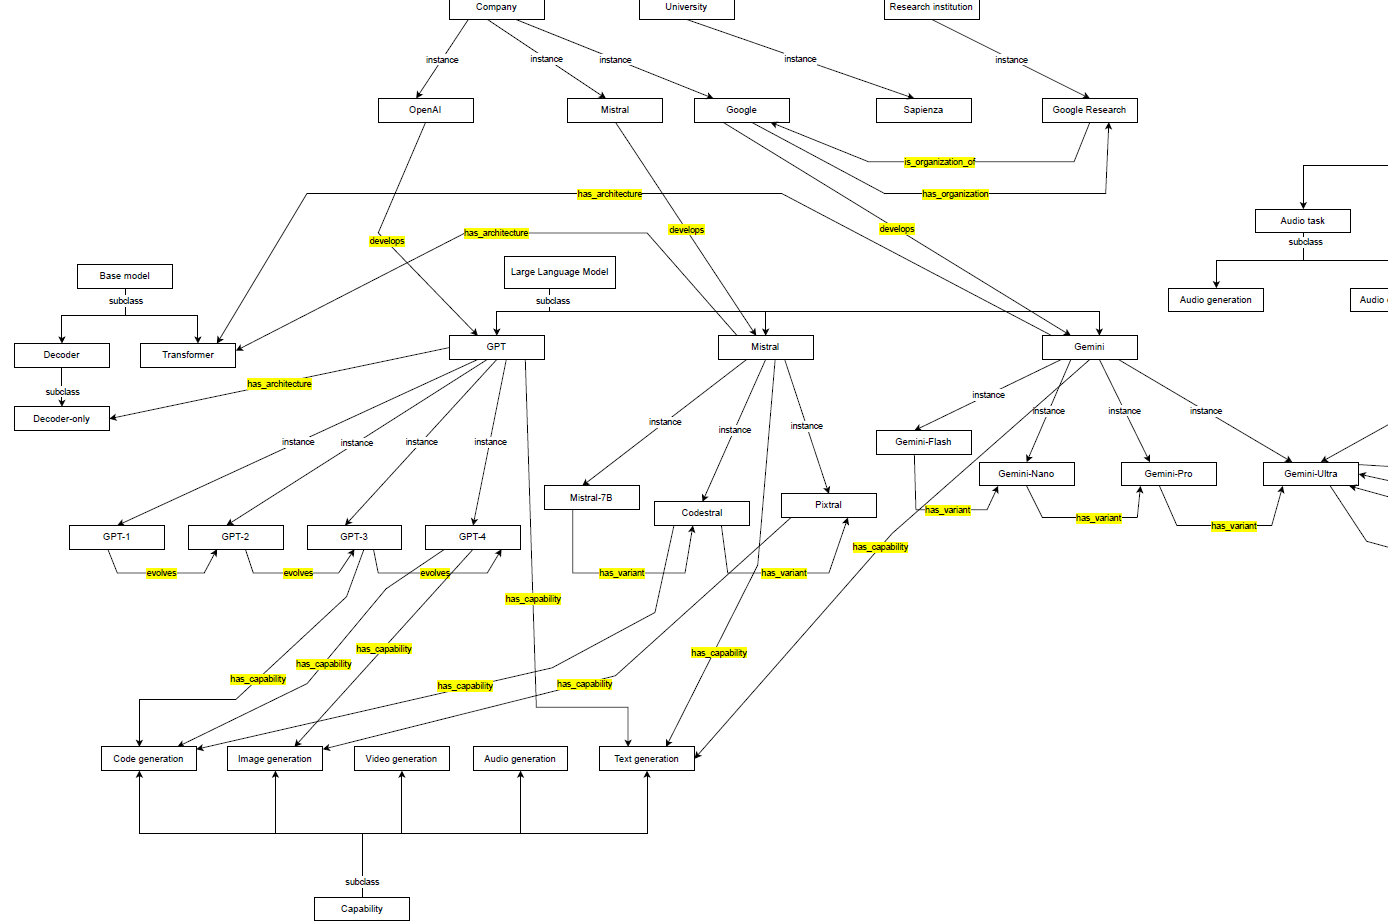
\includegraphics[width=0.9\linewidth]{Figures/fig_26.png}
    \caption{LLMs dimensions conceptualization}
    \label{fig:26}
\end{figure}
The Fig. \ref{fig:26} shows the conceptualization scheme for LLMs.

Regarding the prompt domain, the following relations have been created in order to properly connect the introduced concepts:

\begin{itemize}
    \item solves\_task: connects a prompting technique with a task. The inverse relation is: solved by.

    \item is\_used\_in\_prompt: connects a prompting technique with a prompt. The inverse relation is: prompt generated using.

    \item has\_context: connects a prompt with its context, i.e., a chat where such prompt and possibly more are connected to. The inverse relation is: has prompt.

    \item uses\_model: connects a chat with a LLM that is used to input prompts and generate responses. The inverse relation is: is used in chat.

    \item generates\_response: connects a LLM with the response generated after a prompt to such LLM. The inverse relation is: response generated using.

    \item prompt\_follows\_response: connects a prompt with its response, the inverse relation is: response followed by prompt.

    \item has\_response: connects a chat with a response, the inverse relation is: is response of.
\end{itemize}

\begin{figure}[H]
    \centering
    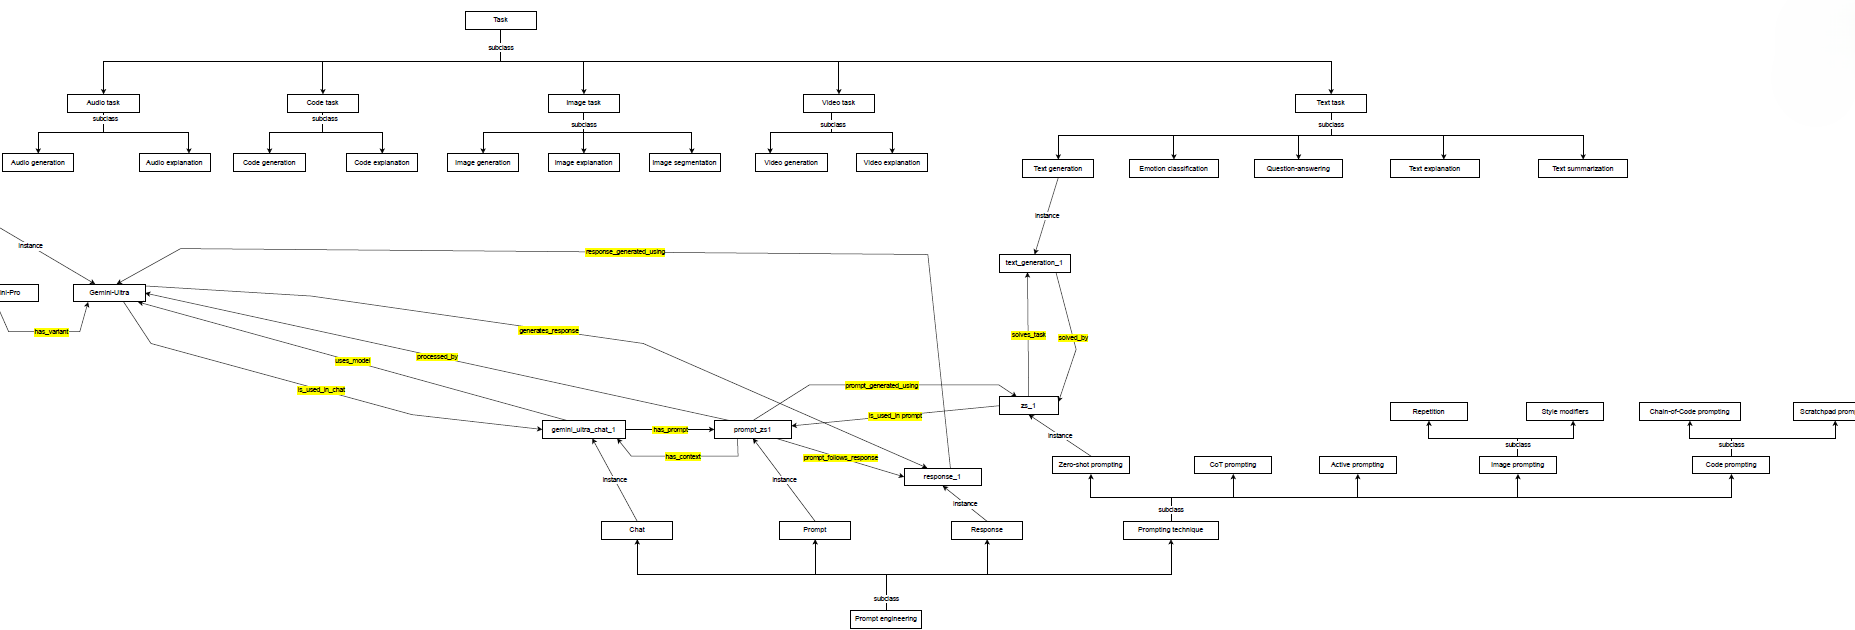
\includegraphics[width=0.9\linewidth]{Figures/fig_27.png}
    \caption{Prompt engineering\\ dimensions conceptualization}
    \label{fig:27}
\end{figure}
The Fig. \ref{fig:27} shows the conceptualization for Prompt Engineering part.

After completing the conceptualization phase, the process can proceed to ontology reuse and ontology encoding.
This involves first identifying similar ontologies within the domain of interest for potential reuse, followed by implementing and encoding the defined concepts using dedicated software tools.

\section{Reuse}
\label{section:4_2_reuse}
Before proceeding with ontology encoding, it is necessary to consider any similar ontologies that can be reused in the creation of the prompt engineering ontology. There are two types of reuse:
\begin{itemize}
    \item Hard reuse: involves directly importing an entire ontology, rigidly incorporating it. Classes and properties are used without modification, ensuring semantic consistency but creating strong dependency on the original ontology.

    \item Soft reuse: involves adapting or copying specific concepts without importing the complete ontology. This approach offers more flexibility, allowing customization, but it may introduce semantic inconsistencies or redundancies 
\end{itemize}

\subsection{Ontology Design Patterns Reuse}
\label{subsection:4_2_1_design_patterns}
During the design of PEO, we decided to use three design patterns:
\begin{itemize}
    \item Description pattern
    \item Sequence pattern
    \item Task Execution
\end{itemize}

The description pattern is used in the definition of subclasses of LLM class, where its subclasses describe the LLM class.\cite{description_pattern}
In fact, this ODP allows the designer to represent both a (descriptive) context and the elements that characterize and are involved in that context.

\begin{figure}[H]
    \centering
    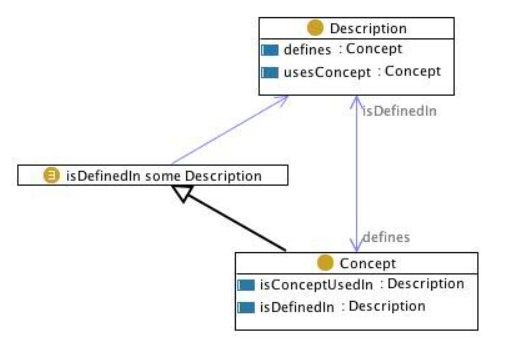
\includegraphics[width=0.6\linewidth]{Figures/fig_73.png}
    \caption{Description pattern}
    \label{fig:73}
\end{figure}
The Fig. \ref{fig:73} shows graphically the Description pattern.

The sequence pattern is used in the ontology to represent evolutionary aspects, specifically among instances of LLMs, involving the relationships evolves and evolves\_from.
This ontology design pattern allows to represent and reason over transitive or intransitive sequences of any kind \cite{sequence_pattern}.
\begin{figure}[H]
    \centering
    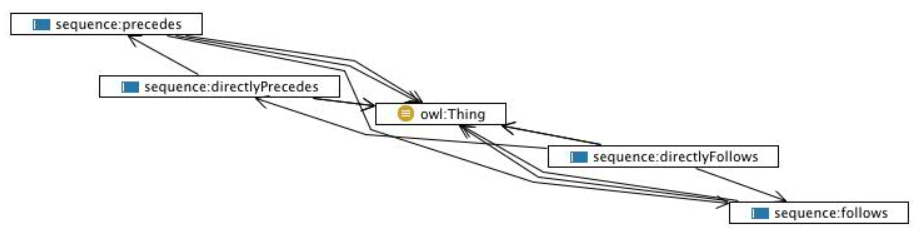
\includegraphics[width=0.8\linewidth]{Figures/fig_74.png}
    \caption{Sequence pattern}
    \label{fig:74}
\end{figure}
The Fig. \ref{fig:74} shows graphically the Sequence pattern.

The task execution pattern is partially used in the representation of task instances executed (solved) by an instance of a prompting technique. More in general, this ODP allows designers to make assertions on roles played by agents without involving the agents that play that roles, and vice versa\cite{task_execution}.

\begin{figure}[H]
    \centering
    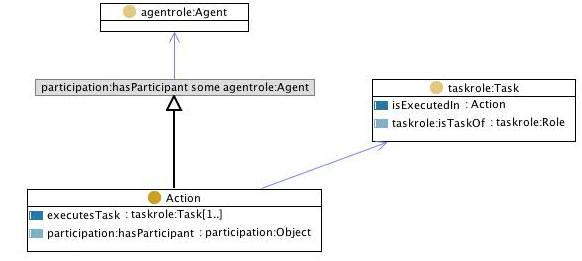
\includegraphics[width=0.8\linewidth]{Figures/fig_75.png}
    \caption{Task Execution}
    \label{fig:75}
\end{figure}
The Fig. \ref{fig:75} shows graphically the Task Execution pattern.

\subsection{State-of-the-art Ontologies Reuse}
\label{subsection:4_2_2_reuse}

I considered two ontologies that can be reused for the implementation of prompt engineering ontology:
\begin{enumerate}
    \item HALO ontology

    \item AI ontology
\end{enumerate}


The HALO ontology \cite{nananukul2024halo}, reviewed in the state-of-the-art chapter, has been considered due to its relevance to a domain closely connected to LLMs, specifically addressing the hallucinations they generate.
The ontology is accessible on GitHub \footnote{https://github.com/navapatn/halo-ontology}.
However, we decide not to reuse it.
This is because it is mostly focused on the hallucinations rather than LLMs and prompts themselves (our target).
Indeed, the class hierarchy on LLMs is shallow in favour of a deeper one on hallucinations.
As such, we deemed the reuse more effortful than the implementation from based on the outcomes of the previous phases that we executed focusing on our target rather than hallucination.
The second ontology considered for reuse is the Artificial Intelligence Ontology \cite{aio}, an ontology that covers machine learning methods, deep learning networks and their components.
This ontology is particularly intriguing, as it stands out as one of the few, if not the only, ontologies focused on the field of artificial intelligence.
It is available on its GitHub repository \footnote{https://github.com/berkeleybop/artificial-intelligence-ontology} in OWL, json and csv format. 
However, we decide not to reuse it, this is because, it mostly is a class hierarchies, while lacking roles.
Moreover, it is focused on machine learning methods.
As such, with the goal of obtaining a broader ontology, it can be seen of an upper level in the hierarchy of LLMs in PEO.
In contrast, PEO describes in more detail LLMs through lower levels in the hierarchy and relationships with the other concepts specific to domain of PEO.


\section{Encoding}
\label{section:4_3_encoding}
\subsection{Software and Tools}
\label{subsection:4_3_1_software}
The ontology encoding phase is where the ontology is actually implemented.
During this stage, the concepts and relationships defined in the conceptualization phase are formalized in OWL. We choose it because it is the standard in the semantic web and it allows to represent complex knowledge by using classes, object properties, data properties, individuals and annotations.

Several tools are available to assist developers with this task.
The main software tools for implementing ontologies include:
\begin{itemize}
    \item Protégé \footnote{https://protege.stanford.edu/}
    \item FluentEditor \footnote{https://www.cognitum.eu/semantics/fluenteditor/}
    \item Vitro \footnote{https://github.com/vivo-project/Vitro?tab=readme-ov-file}
    \item OntoStudio \footnote{https://www.semafora-systems.com/ontobroker-and-ontostudio-x}
\end{itemize}
To begin, we chose Protégé: an open-source ontology editor developed by a team at Stanford University since 1987.
Widely used and highly regarded among ontology engineers, it offers a user-friendly Eclipse-based interface and a wide range of features.

Only a limited number of ontology editors provide an extensive set of features tailored for developers.
Moreover, several editors have remained outdated for years and suffer from lots of bugs.
During the ontology development process, \href{https://git-scm.com/}{Git} was also used: a version control software to track changes made to the ontology that are synchronized with the GitHub repository \footnote{https://github.com/simonegramegna/peo}.
\subsection{First Steps: MetaData and Base Classes}
\label{subsection:4_3_2_encoding}
Starting from an empty page, the first thing to do is the definition of the ontology IRI: which has to be unique and it has to refer to a standard organization.
The ontology IRI of the PEO is: https://w3id.org/peo\#; this IRI will be in every entity created inside the ontology.
\begin{figure}[H]
    \centering
    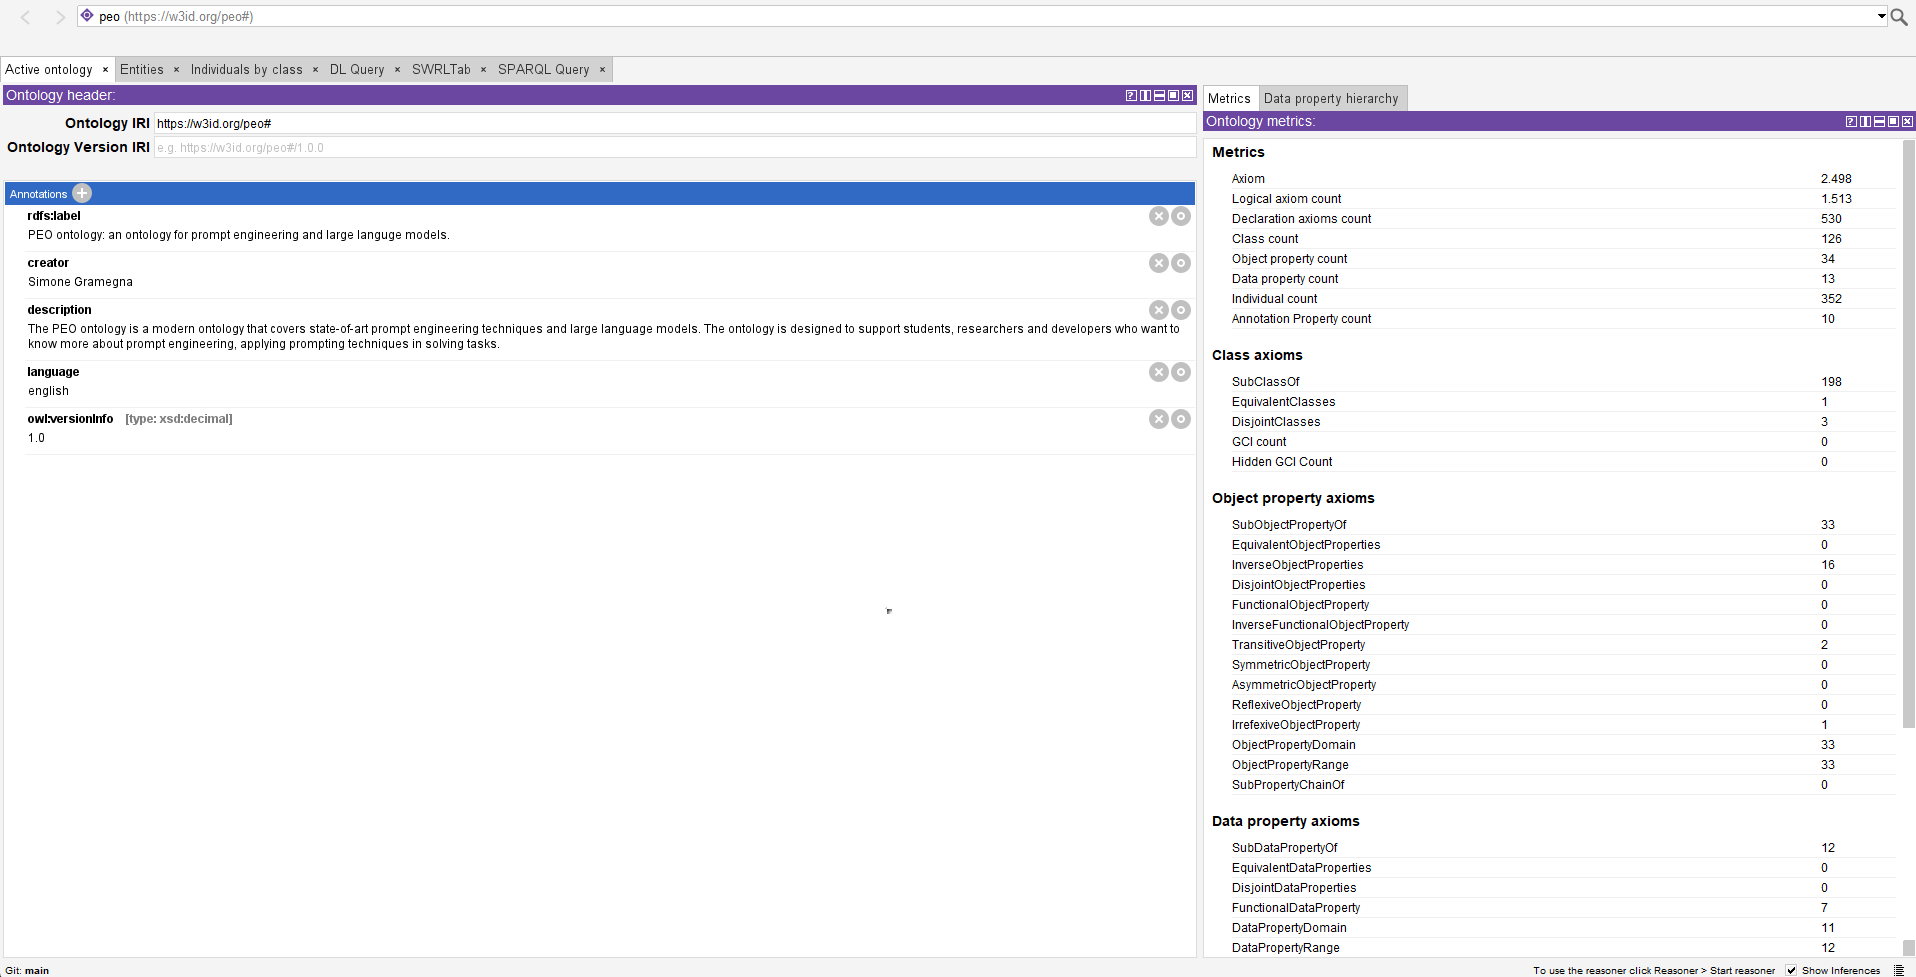
\includegraphics[width=0.8\linewidth]{Figures/fig_29.png}
    \caption{PEO main page}
    \label{fig:29}
\end{figure}
Fig. \ref{fig:29} shows the PEO main page.
Once created the IRI, we define the five annotations and we report them in Tab. \ref{table:t_4_1}. 
\begin{table}[H]
    \footnotesize 
    \centering
    \begin{tabular}{|>{\raggedright\arraybackslash}p{6cm}|>{\raggedright\arraybackslash}p{6cm}|}
        \hline
        Annotation & Annotation value \\ \hline
         rdfs:label & PEO: an ontology for prompt 
         engineering and LLMs. \\ \hline
         
         creator & Simone Gramegna\\ \hline
         
         rdfs:comment & The PEO is a modern ontology that covers state-of-art prompt engineering techniques and LLMs. The ontology is designed to support students, researchers and developers who want to know more about prompt engineering, applying prompting techniques in solving tasks. \\ \hline
         
         language & English \\ \hline
         
         owl:versionInfo & 1.0 \\ \hline
    \end{tabular}
    \caption{Ontology annotations in the main page}
    \label{table:t_4_1}
\end{table}


Starting from the concepts outlined in the conceptualization phase, we define the primary classes of the ontology, which include:
\begin{itemize}
    \item Base model

    \item Capability

    \item Large Language Model

    \item Organization

    \item Prompt engineering

    \item Task
\end{itemize}
All these classes are mutually disjoint, as they represent distinct entities with no overlapping properties.
The only exception is given by "Base model" and "Capability", which are not disjoint.
Both represent attributes of LLMs and are collectively grouped under the "LLM characteristic" class, formed by the union of the two classes. \\
The Capability has five subclasses, each subclass has a label and a comment:
\begin{table}[H]
    \footnotesize 
    \centering
    \begin{tabular}{|>{\raggedright\arraybackslash}p{6cm}|>{\raggedright\arraybackslash}p{6cm}|}
        \hline
        Label & Comment \\ \hline
         Audio processing &  Capability to process audio files. \\ \hline
         
         Code processing & Capability to process source code written in any programming language. \\ \hline
         
         Image processing & Capability to process images, understanding the content of the image. \\ \hline
         
         Text processing & Capability to process text and documents with text inside. \\ \hline
         
         Video processing & Capability to process video files. \\ \hline
    \end{tabular}
    \caption{Capability subclasses}
\end{table}
Each subclass has an individual with the same name, those individuals are created with the aim of assigning a capability to the instances of LLMs that possess it, this aspect will be discussed later.

\subsection{Definition of Large Language Models and their Characteristics}
\label{subsection:4_3_3_llms}
The class "Base model" represents the models at the base of the architecture of LLMs, it has six subclasses each one with label, description and reference.
A subclass can have another subclass representing a more specific architecture, for example the subclass "Decoder" has the subclasses "Decoder only" and "Pixel decoder". 
I have included only the foundational models of the LLMs represented in the ontology, excluding other base models as they fall outside the scope of this ontology.
The subclasses included are: 
\begin{table}[H]
    \footnotesize 
    \centering
    \begin{tabular}{|>{\raggedright\arraybackslash}p{6cm}|>{\raggedright\arraybackslash}p{6cm}|}
        \hline
        Class & Subclasses \\ \hline
         CLIP & none \\ \hline
         
         Decoder & Decoder-only, Pixel decoder \\ \hline
         
         Diffusion model & none \\ \hline
         
         Encoder & Encoder only, Global Image Encoder, Grounding Image Encoder, Region Encoder, ViT Encoder \\ \hline
         
         Recurrent Neural Network & none \\ \hline

        Transformer & Q-Former, LAMDA PT, Transformer XL \\ \hline
    \end{tabular}
    \caption{Base model subclasses}
\end{table}
The class "LLM characteristic" is a subclass of both "Base model" and "Capability".
Each LLM subclass is connected to those two classes using the relations: has\_capability (inverse relation is\_capability) and has\_model\_architecture.
In total there are 33 LLMs subclasses of LLM, each representing a type of LLM such as GPT, Gemini ecc.
The definition of LLMs is completed with a label, a description, a link to the paper, and a link to the website.
Below there are LLMs in PEO with their capabilities and architecture.
\begin{table}[H]
    \footnotesize 
    \centering
    \begin{tabular}{|>{\raggedright\arraybackslash}p{4cm}|>{\raggedright\arraybackslash}p{4cm}|>{\raggedright\arraybackslash}p{4cm}|}
        \hline
        LLM & Capabilities & Base models \\ \hline
        Alpaca & Text processing & Transformer\\ \hline
        BERT & Text processing & Encoder only \\ \hline
        BLIP-2 & Image processing & Q-Former \\ \hline
        BLOOM & Text processing & Transformer \\ \hline
        Chinchilla & Text processing & Transformer \\ \hline
        Claude & Text processing & Transformer \\ \hline
        CogVLM & Image processing & ViT Encoder \\ \hline
        Command R & Text processing & Transformer \\ \hline
        DALL-E & Image processing & CLIP, Decoder, Transformer \\ \hline
        Falcon & Text processing & Decoder only \\ \hline
        FLAN & Text processing & LAMDA PT \\ \hline
        Gemini & Audio processing, Code processing, Image Processing, Text processing, Video processing & Transformer\\ \hline
        Gemma & Text processing & Transformer \\ \hline
        GLaMM & Image processing & Global Image Encoder, Grounding Image Encoder \\ \hline
        LLaMA & Text processing & Transformer \\ \hline
        Midjourney & Image processing & Diffusion model  \\ \hline
        Minerva & Text processing & Transformer \\ \hline
        Mistral & Text processing & Transformer \\ \hline
        MPT-7B & Text processing & Decoder only \\ \hline
        OLMo & Text processing & Decoder only \\ \hline
        OpenELM & Text processing & Decoder only \\ \hline
        OPT & Text processing & Transformer \\ \hline
        PaLM & Text processing, Code processing & Transformer \\ \hline
        Phi-1 & Text processing & Transformer \\ \hline
        RWKV LLM & Text processing & Recurrent Neural Network, Transformer \\ \hline
        Sora & Video processing & Decoder only \\ \hline
        StableLM & Text processing & Decoder only \\ \hline
        StarCoder & Code processing & Decoder only \\ \hline
        T5 & Text processing & Transformer \\ \hline
        VALL-E & Audio processing & Transformer \\ \hline
        Vicuna & Text processing & Transformer \\ \hline
        XLNet & Text processing & Transformer XL \\ \hline
    \end{tabular}
    \caption{Large language models in PEO}
\end{table}
There is a relation based\_on between two subclasses of LLM (with inverse relation basis\_for) where a LLM is developed starting from the base of another LLM.
For example Alpaca is based on LLaMA (another family of LLMs).
Each type of LLM has a capability, this capability is common for all instances of the LLM.
Hence, if a specific version of a LLM has a new capability, the single LLM can be connected to that specific capability. For example, GPT has capability text processing but GPT-3.5 has also the capability of code processing so this version has two capabilities (text processing and code processing).
Same goes for GPT-4 which is an evolution of GPT-3.5 and has also the image processing capability; so it has three capabilities (text processing, code, processing and image processing).
This approach is very flexible because there is no need to divide into categorical classes each version of LLM by simply connecting the version with the specific instance of the capability.
There are three relations between versions of the same LLM: 
\begin{itemize}
    \item has\_variant: relation between two LLMs (x and y), where x has y as another version.

    \item evolves: transitive relation between two LLMs (x and y), where y is an evolution of x. 

    \item evolved\_from: transitive inverse relation of evolves between two LLMs x and y.
\end{itemize}

The relation has\_variant express a different version of the model, while the relation evolves specifies the evolution between two LLMs. 
The latter can also be used to infer the former.
For example, if GPT-3.5 evolves GPT-4 then GPT-3.5 has variant GPT-4.
We use SWRL rules to infer this connection. 
The chosen reasoner is the Hermit reasoner\cite{glimm2014hermit}: a reasoner already included in Protégé which does not require the installation of any additional plug-in.
The reasoner ensures the ontology consistency, inferring new axioms and processing SWRL rules.

SWRL rules are widely applied in PEO.
Firstly, they can infer the relation has\_variant from the relation  evolves. Specifically, the rule is:
\begin{lstlisting}
peo:evolves(?x, ?y) -> peo:has_variant(?x, ?y)
\end{lstlisting}
$?x$ and $?y$ are the two instances involved in the relations.
The rule is applied to all instances that satisfy the condition in the body of the rule.
If a model evolves into another model, the evolved model has the capabilities of the previous model.
This concept is expressed using this SWRL rule:
\begin{lstlisting}
peo:evolves(?x, ?y) ^ peo:has_capability(?x, ?c) -> peo:has_capability(?y, ?c)
\end{lstlisting}
These two relations are not explicitly defined in the ontology, but are inferred by the reasoner.
Each instance of the LLM has two data properties associated 
\begin{itemize}
    \item has\_number\_parameters: number of parameters of the model.

    \item has\_release\_year: year of release of the model
\end{itemize}
Those two data properties are functional, assigning a single value of each property to the instance of the LLM.

Large language models are developed by organizations that can be universities, research institutions and companies for business purpose, the class Organization contains has such three subclasses (with label  and description).
\begin{table}[H]
    \footnotesize 
    \centering
    \begin{tabular}{|>{\raggedright\arraybackslash}p{6cm}|>{\raggedright\arraybackslash}p{6cm}|}
        \hline
        Subclass or organization & Number of entities \\ \hline
        
        University & 2 \\ \hline
 
        Research institution & 8 \\ \hline
        
        Company & 13 \\ \hline
    \end{tabular}
    \caption{Number of organization entities}
\end{table}
Every instance of organization has two associated data properties:
\begin{itemize}
    \item registered\_name: the official name of the organization.

    \item official\_website: the official website of the organization.
\end{itemize}
Organizations and LLMs are connected using the develops relation, connecting an organization with an LLM. 
It is well known that an organization not only develops a single version of an LLM, but the entire family (represented by the different subclasses of the LLM class).
Based on the relation has\_variant, we created the following SWRL rule
\begin{lstlisting}
peo:develops(?c, ?x) ^ peo:has_variant(?x, ?y) -> peo:develops(?c, ?y)    
\end{lstlisting}
If a company $c$ develops a LLM $?x$ and the LLM $x$ has variant another LLM (of the same type) $y$, then the company $c$ develops the llm $y$.
This rule requires that the relationship has\_variant exists among all versions of LLMs or the relation evolves should exist, in order to infer has\_variant.
For example, if OpenAI develops GPT-1, GPT-1 evolves GPT-2 (has variant GPT-2) then OpenAI develops GPT-2.
This process during the inference is automatic because the evolves relation is transitive.

Another SWRL rule that involves the develops relation is the following:
\begin{lstlisting}
peo:is_organization_of(?o1, ?o2) ^ peo:develops(?o1, ?llm) -> peo:develops(?o2, ?llm)
\end{lstlisting}
If an organization $o1$ is organization of another organization $o2$ (for example DeepMind is organization of Google) and $o1$ develops a LLM, then $o2$ develops the LLM.
This is important to specify because several research teams rely on and acknowledge the contribution of other organizations that provides financial support and resources.

\subsection{Definition of Task}
\label{subsection:4_3_4_task}
The Task class represents task that are solved by LLMs applying prompting techniques, there are five specific subclasses representing the different types of task distinguished based on the type of data to process: image, text, video, audio, or code.
Each subclass has other subclasses representing the specific task, e.g., audio generation, text translation ecc as we can see in the table below:
\begin{table}[H]
    \footnotesize 
    \centering
    \begin{tabular}{|>{\raggedright\arraybackslash}p{6cm}|>{\raggedright\arraybackslash}p{6cm}|}
        \hline
        Task type & Subclasses \\ \hline
        Audio task & Audio generation, Audio explanation \\ \hline

        Video task & Video generation, Video explanation \\ \hline
    \end{tabular}
    \caption{Types of task with subclasses - part 1}
\end{table}

\begin{table}[H]
    \footnotesize 
    \centering
    \begin{tabular}{|>{\raggedright\arraybackslash}p{6cm}|>{\raggedright\arraybackslash}p{6cm}|}
        \hline
        Task type & Subclasses \\ \hline
        Code task & Code generation, Code explanation \\ \hline

        Image task & Image generation, Image explanation, Image segmentation \\ \hline

        Text task & Emotion classification, Mathematical understanding, Question-Answering, Text explanation, Test generation, Text summarization, Text translation \\ \hline
    \end{tabular}
    \caption{Types of task with subclasses - part 2}
\end{table}
All of those classes have a label and a description describing shortly the task.
The data property has\_description can be employed for a task to specify its description.

\subsection{Definition of Prompt Engineering}
\label{subsection:4_3_5_prompt}
The Prompt engineering class serves to model all concepts associated with prompts, such as their creation, the context in which they are applied, and the responses they produce.
It has four main subclasses, each one with a label and a description:
\begin{itemize}
    \item Chat: context in which a prompt is created. 
    \item Prompt: input to a LLM.
    \item Prompting technique: technique used to create a prompt.
    \item Response: response given by a LLM after a prompt.
\end{itemize}
The prompting technique is very important because it has all the subclasses representing the different prompting techniques and all instances of those classes are connected using different object properties.
All subclasses of Prompting Technique refer to techniques used in tasks that involve processing only textual content.
Prompting techniques related to images and source code are specifically addressed by their respective class hierarchies based on Code prompting technique and Image prompting techniques.
Prompting techniques for audio and video have not been specified, as the few existing techniques are not yet well-established.
The prompting techniques are gathered from papers, as seen in the background chapter, each subclass representing the specific technique has a label, a description and a reference.
In total there are 24 prompting techniques:
\begin{itemize}
    \item Active prompting 
    \item Analogical prompting
    \item Automatic Chain-of-Thought prompting
    \item Chain-of-Knowledge prompting
    \item Chain-of-Note prompting
    \item Chain-of-Table prompting
    \item Chain-of-Thought prompting
    \item Chain-of-Verification prompting
    \item Decomposed prompting
    \item Emotion prompting
    \item Few shot prompting
    \item Graph of Thoughts prompting
    \item Least-to-most prompting
    \item Logical Chain-of-Thought prompting
    \item ReAct prompting
    \item Retrieval Augmented Generation - RAG prompting
    \item Role prompting
    \item Self consistency prompting
    \item System-2-Attention prompting
    \item Take a step back prompting
    \item Thread of Thought prompting
    \item Tree of Thoughts prompting
    \item Zero shot prompting
\end{itemize}
For code, the class Code Prompting Technique has four subclasses:
\begin{itemize}
    \item Chain-of-Code prompting
    \item Program of Thoughts prompting
    \item Scratchpad prompting
    \item Structured Chain-of-Thought prompting
\end{itemize}
Image prompting technique class has six subclasses:
\begin{itemize}
    \item Fix deformed generations prompting
    \item Lighting
    \item Quality boosters
    \item Repetition
    \item Shot type
    \item Style modifiers
\end{itemize}
To ensure the accurate and consistent representation of prompts generated using the listed techniques, instances of the Prompting Technique class are connected to instances of other Prompt Engineering subclasses via dedicated object properties, defined explicitly or inferred by the reasoner using SWRL rules.
To illustrate all instances along with their associated object properties and data properties, we propose a simple task: translating the phrase "Ciao, come va?" from Italian to English using a zero-shot prompt as input to GPT-4.\\
The first step is to create, if it does not already exist, an instance of the "Text translation" subclass of Task, which we will name "translation\_1" assigning for the data property has\_description the string value: "Translation of the text: Ciao, come va?".
Now I create the instance of the prompting technique that is going to solve the task, in this case we create an instance of the subclass "Zero shot prompting" called "zs\_prompting\_1".
This instance is connected to "translation\_1" using the object property solves\_task with the inverse property "solved\_by" connecting the two instances in both directions. Before creating the prompt, we create an instance of the chat class, calling it "gpt4\_chat\_1" and connecting to the instance GPT-4 of the GPT class using the object property uses\_model with inverse property is\_used\_in\_chat.
The chat instance has three data properties associated:
\begin{itemize}
    \item has\_chat\_title: title of the chat, we assign it "Translation GPT-4 italian to english 1".

    \item start\_time\_chat: start time of the chat, we assign to it the currant time while I'm writing this chapter: "29/11/2024 - 10:37"

    \item end\_time\_chat: end time of the chat, the chat has the duration of two minutes and I assign the value: "29/11/2024 - 10:39"
\end{itemize}
Obviously those example values can be modified later.
Now that a context is established, the chat "gpt4\_chat\_1", we proceed to create the instance of the Prompt.
We specify that the prompt called "zs\_1" is created using the instance of Zero shot prompting previously defined using the object property prompt\_generated\_using with inverse property is\_used\_in\_prompt, in our case "zs\_1" is generated using "zs\_prompting\_1".
A prompt instance can have three associated data properties:
\begin{itemize}
    \item has\_instruction: main instruction of the prompt.

    \item has\_input\_data: data given as input to the prompt. 

    \item has\_output\_indicator: indicator that indicates the format of the response.
\end{itemize}
For simplicity, we assign the instruction "Translate the English text to Italian, the input Text: Ciao, come va?  and the output format: Translation:  to the prompt, other data properties values can be added later.
Now we connect the prompt with its context, the "gpt4\_chat\_1" using the object property has\_context with inverse relation has\_prompt and after the creation of this relation using a SWRL rule I connect the prompt with the LLM that takes it in input. 
\begin{lstlisting}
peo:has_context(?p, ?c) ^ peo:uses_model(?c, ?m) -> peo:processed_by(?p, ?m)   
\end{lstlisting}
If the context of a prompt $p$ is a chat $c$, which uses the LLM $m$, then $p$ is processed by the LLM $m$.
This rule creates automatically during the reasoning the relation processed\_by with inverse relation processes.

After a prompt, the LLM generates a response, which in PEO is instance of the Response class.
The value is associated using the data property has\_response\_value and is connected to the prompt that generated it using the object property response\_followedby\_prompt.
In order to model the "chain" prompt-responses-prompt, I created the following object properties:
\begin{itemize}
    \item response\_followedby\_prompt: the response is after a prompt.

    \item prompt\_follows\_response: after the prompt there is a response, inverse property of response\_followedby\_prompt.

    \item prompt\_follows\_prompt: after the prompt there is another prompt.

    \item prompt\_followedby\_prompt: before the prompt there is another prompt, inverse property of {prompt\_follows\_prompt}.

    \item response\_follows\_prompt: after the response there is a prompt.

    \item prompt\_followedby\_response: before the prompt there is a response, inverse relation of response\_follows\_prompt. 
\end{itemize}
We can graphically see this concatenation in the following scheme:
\begin{figure}[H]
    \centering
    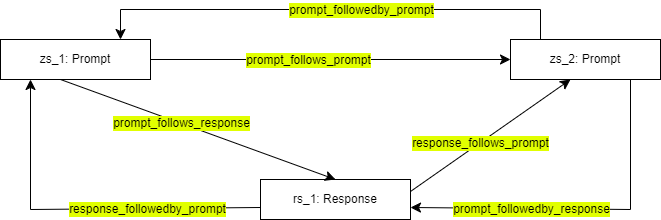
\includegraphics[width=0.9\linewidth]{Figures/fig_30.png}
    \caption{Chain prompt-response}
    \label{fig:enter-label}
\end{figure}
Of course, most of these relationships are automatically created during the inference process.
To connect a response with the next prompt, we created this SWRL rule:
\begin{lstlisting}
peo:prompt_followedby_prompt(?x, ?y) ^ peo:prompt_follows_response(?y, ?r) -> peo:prompt_followedby_response(?x, ?r)
\end{lstlisting}
It states that if a prompt $?x$ is followed by another prompt $?y$ and $?y$ has a response $?r$, then $?x$ is followed by $?r$.

The context of the next prompt is assigned automatically using the object property prompt\_followedby\_prompt and this SWRL rule:
\begin{lstlisting}
peo:prompt_followedby_prompt(?x, ?y) ^ peo:has_context(?y, ?c) -> peo:has_context(?x, ?c)
\end{lstlisting}
It states that if a prompt $x$ is followed by another prompt $y$ and $y$ is connected to the chat $c$ as context, then $x$ has context $c$.
Also, each response is connected the chat using the object property is\_response\_of (inverse property has\_response) created using the SWRL rule:
\begin{lstlisting}
peo:response_followedby_prompt(?r, ?p) ^ peo:has_context(?p, ?c) -> peo:is_response_of(?r, ?c)
\end{lstlisting}
It states that if a response $?r$ is followed by a prompt $?p$, which is connected to the chat $c$ as context, then the response $?r$ is the response of $?c$.
The last SWRL rule connects the response with the model that has generated it creating the object property response\_generated\_using with the inverse property generates\_response:
\begin{lstlisting}
peo:response_followedby_prompt(?r, ?p) ^ peo:processed_by(?p, ?m) -> peo:response_generated_using(?r, ?m) 
\end{lstlisting}
It states that if a response $?r$ is followed by a prompt $?p$ and the prompt $?p$ is processed by the LLM $?m$, then the response $?r$ is generated using $?m$.
\begin{figure}[H]
    \centering
    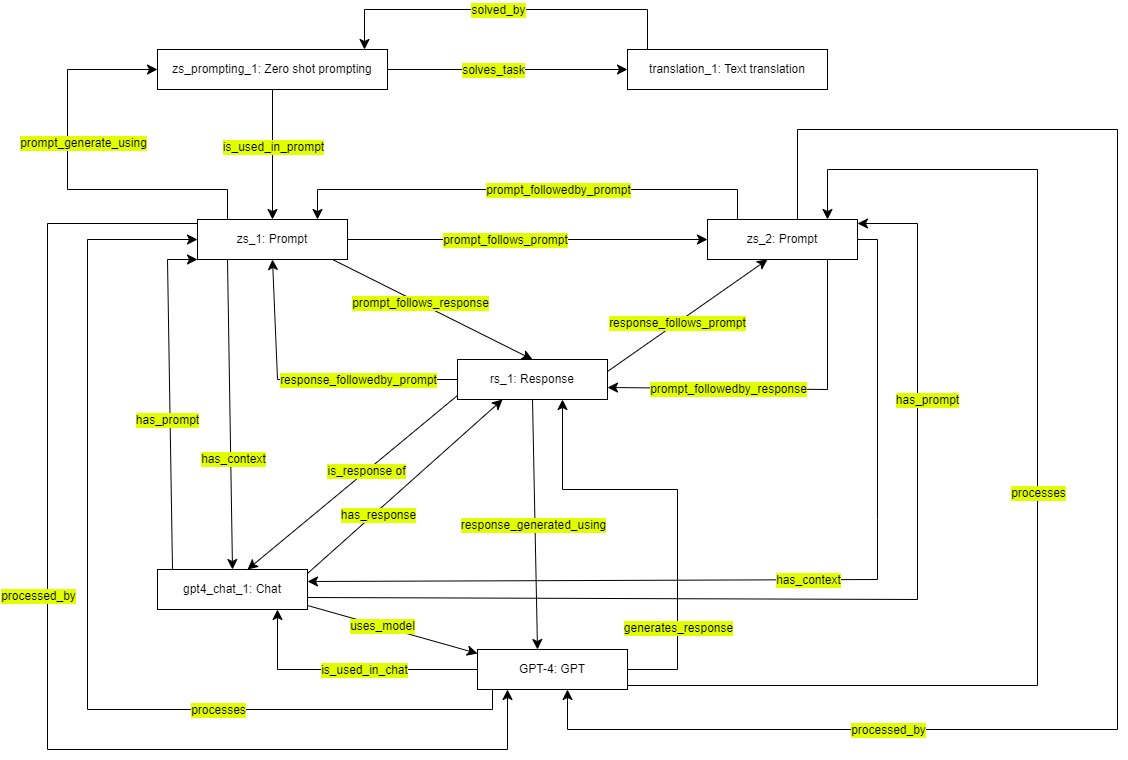
\includegraphics[width=0.85\linewidth]{Figures/fig_31.png}
    \caption{Chat scheme}
    \label{fig:31}
\end{figure}
Fig.~\ref{fig:31} further clarifies the aforementioned object properties.

\subsection{Population}
\label{subsection:4_3_6_population}
Populating the ontology with prompts is a complex process as it requires connecting various instances (task, prompting technique, prompt, chat, response, LLM) using the defined object properties. Moreover, each prompt is manually crafted in accordance with the specific prompting technique.
Manually populating the ontology with all instances for every task, every version of each LLM, and every prompting technique would be highly time-consuming and beyond the objectives of this thesis.
Therefore, we focus on a specific subset of the ontology: LLMs, tasks, prompting techniques, and prompts.
The LLMs are very popular ones available to the users, namely:
\begin{itemize}
    \item GPT-4
    \item Mistral-7B
    \item Gemini Flash
\end{itemize}
Moreover, the following prompting techniques are considered:
\begin{itemize}
    \item Zero-shot prompting: allows LLMs to handle new tasks using only natural language instructions, without requiring examples or any effort by the user.

    \item Few-shot prompting: enables language models to learn new tasks with few examples, reducing the need for extensive task-specific datasets.
    
    \item Role prompting: improves LLMs performance on solving tasks by simulating specific roles.

    \item Emotion prompting:  enhances LLMs by integrating emotions into prompts, improving response generation and performance on tasks.

    \item Analogical prompting: is able to generate automatically task-specific exemplars, reducing manual annotation needs, and improving performance on problem-solving tasks.
\end{itemize}
Finally, the following four tasks are considered:
\begin{itemize}
    \item Emotion classification: classification of the emotion in a given text.

    \item Mathematical understanding: solving a given mathematical problem of medium difficulty. 

    \item Text translation: translation of a text from English to Italian.

    \item Text summarization: summarization of the content of a given text.
\end{itemize}

Below, we list the prompts created for each task and for each prompting technique.\\\\
Task 1: Emotion classification\\     
The input text to be classified is: "I think the vacation is okay"
\begin{itemize}
    \item Zero-shot prompting: Classify the text into neutral, negative or positive. Text: "I think the vacation is okay." Sentiment:
    \item Few-shot prompting: Classify the following text into neutral, negative, or positive based on its sentiment. Here are some examples: 
    Text: "The food was absolutely wonderful!" Sentiment: Positive. 
    Text: "I did not enjoy the movie at all." Sentiment: Negative. 
    Text: "It was an average experience." Sentiment: Neutral. 
    Now, classify this text: Text: "I think the vacation is okay." Sentiment:
    \item Emotion prompting: Classify the following text into neutral, negative, or positive based on its sentiment. This task is very important to my career. Please provide a well-thought and accurate classification. Text: "I think the vacation is okay." Sentiment:
    \item Role prompting: From now on, you are an experienced sentiment analyst with deep expertise in understanding human emotions through textual analysis. Your task is to classify the sentiment of texts as neutral, negative, or positive with utmost accuracy and professionalism. Text: "I think the vacation is okay." Sentiment:
    \item Analogical prompting: Classify the text into neutral, negative or positive. \# Instruction: \# Text: I think the vacation is okay. \# Sentiment:
\end{itemize}
Task 2: Mathematical understanding\\
For the mathematical understanding there is the solving of a simple geometrical problem: the calculation of a square with the four vertices at (-2, 2), (2, -2), (-2, -6), and (-6, -2). 
\begin{itemize}
    \item Zero-shot prompting: What is the area of the square with the four vertices at $(-2, 2)$, $(2, -2)$, $(-2, -6)$, and $(-6, -2)$?
    \item Few-shot prompting: Instruction: Determine the area of a square given the coordinates of its four vertices. 
    Example 1: Vertices: $(0, 0)$, $(4, 0)$, $(4, 4)$, $(0, 4)$ 
    Step 1: Identify the side length. Distance between $(0, 0)$ and $(4, 0)$ is $\sqrt{((4 - 0)^2 + (0 - 0)^2)} = 4$. 
    Step 2: Calculate the area. Area = side length$^2 = 4^2 = 16$. Answer: 16. 
    Example 2: Vertices: $(-1, 1)$, $(-1, 3)$, $(1, 3)$, $(1, 1)$ 
    Step 1: Identify the side length. Distance between $(-1, 1)$ and $(-1, 3)$ is $\sqrt{((3 - 1)^2 + (1 - 1)^2)} = 2$. 
    Step 2: Calculate the area. Area = side length$^2 = 2^2 = 4$. Answer: 4. 
    Query: Vertices: $(-2, 2)$, $(2, -2)$, $(-2, -6)$, $(-6, -2)$. 
    Step 1: Identify the side length by calculating the distance between consecutive vertices. 
    Step 2: Calculate the area of the square. Answer:
    \item Emotion prompting: Please calculate the area of a square given the coordinates of its vertices. This task is important for building my understanding of geometry and improving my analytical skills, so I truly value a thorough and accurate solution. Vertices: $(-2, 2)$, $(2, -2)$, $(-2, -6)$, $(-6, -2)$.
    \item Role prompting: From now on, you are a brilliant geometry teacher. You always explain geometry problems thoroughly and ensure your students understand every step of the process. We have a question for you: I have four vertices of a square: $(-2, 2)$, $(2, -2)$, $(-2, -6)$, and $(-6, -2)$. Can you help me calculate the area of the square step by step? Please provide a detailed explanation of how to verify the shape, calculate the side length, and determine the area.
    \item Analogical prompting: What is the area of the square with the four vertices at $(-2, 2)$, $(2, -2)$, $(-2, -6)$, and $(-6, -2)$? \# Instruction: \#\# Recall relevant exemplars: \#\# Solve the initial problem:
\end{itemize}
Task 3: Text translation\\
For text translation task I chosed a citation of Lewis Carol \cite{carol} to translate form english to italian: "Sometimes, we've believed as many as six impossible things before breakfast."
\begin{itemize}
    \item Zero-shot prompting: Translate the English text to Italian. Text: "Sometimes, we've believed as many as six impossible things before breakfast." Translation:
    \item Few-shot prompting: Translate the following English sentences into Italian: 
    1. English: "Sometimes, we've believed as many as six impossible things before breakfast." Italian: "A volte, ho creduto a ben sei cose impossibili prima di colazione." 
    2. English: "I think, therefore I am." Italian: "Penso, quindi sono." 
    3. English: "All the world's a stage, and all the men and women merely players." Italian: "Tutto il mondo è un palcoscenico e tutti gli uomini e le donne sono solo attori." 
    Now translate this sentence: English: "Sometimes, we've believed as many as six impossible things before breakfast." Italian:
    \item Emotion prompting: Translate the following text to Italian. It's very important for me to understand this translation accurately as it could affect my professional progress: "Sometimes, we've believed as many as six impossible things before breakfast."
    \item Role prompting: From now on, you are an excellent literary translation teacher who accurately explains the meaning and tone of complex sentences. Translate the following sentence from English to Italian, preserving its meaning and tone: "Sometimes, we've believed as many as six impossible things before breakfast."
    \item Analogical prompting: \# Problem: "Sometimes, we've believed as many as six impossible things before breakfast." 
    \# Relevant Problems: 
    1. Translating a complex sentence from English to Italian. 
    - Question: How to translate the sentence "To be or not to be, that is the question" into Italian? 
    - Answer: The sentence "To be or not to be, that is the question" translates into Italian as "Essere o non essere, questo è il problema." 
    2. Translating a sentence with idiomatic expressions. 
    - Question: How to translate "Break a leg!" into Italian? 
    - Answer: The idiomatic expression "Break a leg!" translates into Italian as "In bocca al lupo!" 
    3. Translating a sentence with abstract concepts. 
    - Question: How to translate "The only limit is your imagination" into Italian? 
    - Answer: The sentence "The only limit is your imagination" translates into Italian as "L'unico limite è la tua immaginazione." 
    \# Translation of the initial problem: The sentence "Sometimes, we've believed as many as six impossible things before breakfast" translates into Italian as:
\end{itemize}
Task 4: Text summarization\\
The last task is the summarization of the following text about permaculture: "Permaculture is a design process mimicking the diversity, functionality and resilience of natural ecosystems. The principles and practices are drawn from traditional ecological knowledge of indigenous cultures combined with modern scientific understanding and technological innovations. Permaculture design provides a framework helping individuals and communities develop innovative, creative and effective strategies for meeting basic needs while preparing for and mitigating the projected impacts of climate change."\cite{permaculture}
\begin{itemize}
    \item Zero-shot prompting: Permaculture is a design process mimicking the diversity, functionality and resilience of natural ecosystems. The principles and practices are drawn from traditional ecological knowledge of indigenous cultures combined with modern scientific understanding and technological innovations. Permaculture design provides a framework helping individuals and communities develop innovative, creative and effective strategies for meeting basic needs while preparing for and mitigating the projected impacts of climate change. Write a summary of the above text. Summary:
    \item Few-shot prompting: You are an expert at creating concise summaries. Below are some examples of summaries based on texts.
    Example 1: Text: The Earth orbits the Sun in an elliptical pattern, taking approximately 365.25 days to complete one orbit. This forms the basis of the Gregorian calendar year. Summary: The Earth completes an orbit around the Sun in roughly 365 days, defining the calendar year.
    Example 2: Text: Sustainable agriculture incorporates practices that maintain productivity and minimize environmental impact, such as crop rotation and organic farming. Summary: Sustainable agriculture uses eco-friendly practices like crop rotation and organic methods to maintain productivity.
    Task: Text: Permaculture is a design process mimicking the diversity, functionality, and resilience of natural ecosystems. The principles and practices are drawn from traditional ecological knowledge of indigenous cultures combined with modern scientific understanding and technological innovations. Permaculture design provides a framework helping individuals and communities develop innovative, creative, and effective strategies for meeting basic needs while preparing for and mitigating the projected impacts of climate change. Summary:
    \item Emotion prompting: Summarize the essence of permaculture, focusing on its innovative design process inspired by natural ecosystems. Highlight how it combines traditional ecological knowledge with modern science and technology to address climate change. This understanding is vital to my research and the future of sustainable living. Please ensure the summary is concise yet comprehensive.
    \item Role prompting: From now on, you are an environmental scientist who specializes in explaining complex ecological concepts in an accessible and engaging manner. Your task is to provide a concise summary of permaculture principles and their importance in addressing climate challenges.
    \item Analogical prompting: Problem: Summarize the definition and essence of permaculture using principles that mirror natural ecosystems and combine traditional ecological knowledge with modern science. Instruction: Recall three relevant and distinct problems or topics related to summarizing processes that focus on mimicking complex systems. Provide detailed exemplars for each recalled instance, including how the principles were extracted and utilized effectively. Use the recalled insights to structure and write the final summary.
\end{itemize}
The responses for each prompt from the three LLMs have been saved in the ontology, and a chat has been created for each prompt, including a title, start time, and end time resulting in a total of 60 distinct chats.
\begin{figure}[H]
    \centering
    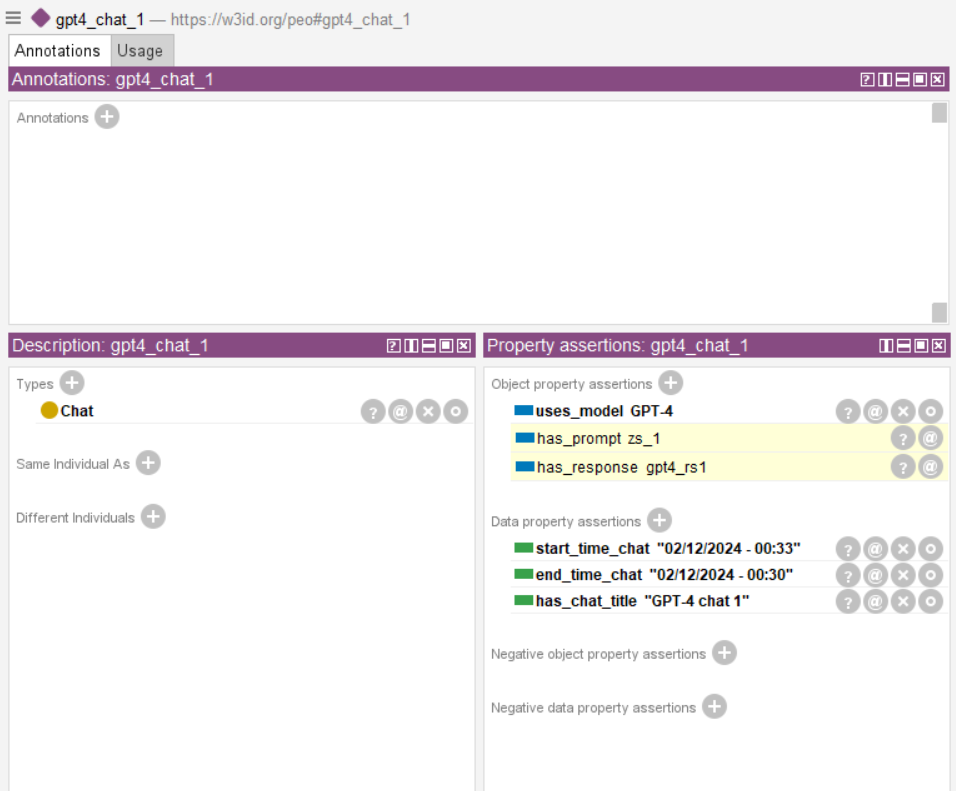
\includegraphics[width=0.75\linewidth]{Figures/fig_32.png}
    \caption{Example of chat with relations inferred}
    \label{fig:enter-label}
\end{figure}

\subsection{Automatic Population}
\label{subsection:4_3_7_automatic}
Populating an ontology with various instances can be a time-consuming task for developers, as the ontology's domain of interest often involves numerous entities requiring manual insertion.
To streamline this process automation can be employed.
The methodology proposed in \cite{norouzi2024ontology} allows to semi-automatically populate modular ontologies using LLMs.
It focuses on leveraging the strengths of LLMs, such as GPT-4 and Llama-3, for extracting structured knowledge from natural language texts.
The method is divided into three main stages: data preprocessing, relevant text retrieval, and ontology population.
In the first stage, the data is cleaned, organized, and aligned with simplified ontology modules to facilitate processing.
The second stage employs text summarization and Retrieval-Augmented Generation (RAG) techniques to identify and extract relevant information aligned with the ontology schema.
Finally, in the third stage, predefined module files guide the LLMs to populate the ontology with accurate triples by using structured prompts.
Despite the good results, the methodology still requires effort, as documents need to be selected and preprocessed to create a dataset that serves as input for the LLM used to populate the ontology. Implementing this process demands skills that go beyond those of an ontology engineer, effectively shifting the workload to another task.\\ 

Moreover, the approach proposed in \cite{saetia2024financial} leverages LLMs, such as GPT-3.5 and GPT-4, to populate financial ontologies by extracting structured data from unstructured texts.
It combines several prompting techniques to improve accuracy and scalability.
Few-shot prompting provides positive and negative examples, whilst Chain-of-Thought (CoT) reasoning encourages step-by-step problem solving,
Moreover, schema.org definitions are included to contextualize fields and properties.
Prompts are carefully designed to generate structured outputs in JSON format for easy integration and evaluating performance using F1 scores, with the best results achieved when combining examples, CoT, and definitions.
Like the previous one, this approach requires considerable effort on gathering necessary docs to pre-process.
Moreover, the quality of the output depends on the prompts.\\
Since our goal in populating the ontology is a set of individuals and triples that is sufficient for the evaluation phase rather than the full range of knowledge, we employ a straightforward ad-hoc approach.
Starting from the sixteen CQs defined in the Ontology requirements specification section, we input them, along with the ontology TBox, into a LLM to generate an automatically populated version of the prompt engineering ontology.
The LLM chosed is GPT-4o: the latest and most powerful version of GPT available in its web interface ChatGPT and used previously in the manual ontology population.
This time instead of giving as input a specific prompt created with one of prompt engineering techniques, we write this prompt, providing the ontology and a text file containing the competency questions.
\begin{figure}[H]
    \centering
    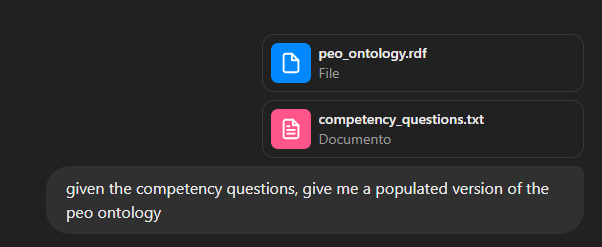
\includegraphics[width=0.9\linewidth]{Figures/fig_34.png}
    \caption{Prompt for automatic ontology population}
    \label{fig:34}
\end{figure}
After this prompt the LLM begins a reasoning process, first it explains the approach followed by the model:
\begin{figure}[H]
    \centering
    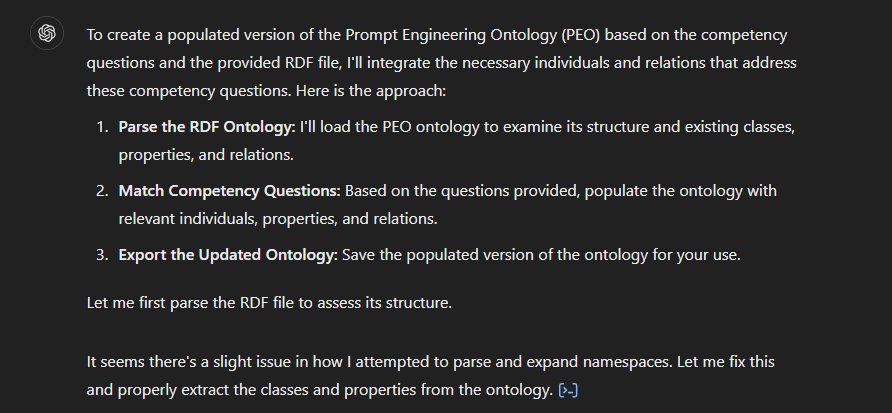
\includegraphics[width=0.9\linewidth]{Figures/fig_35.png}
    \caption{First GPT-4 output in the automatic population}
    \label{fig:enter-label}
\end{figure}
Then the model analyses the ontology structure encoded in the RDF file, listing simple classes and sample object properties found:
\begin{figure}[H]
    \centering
    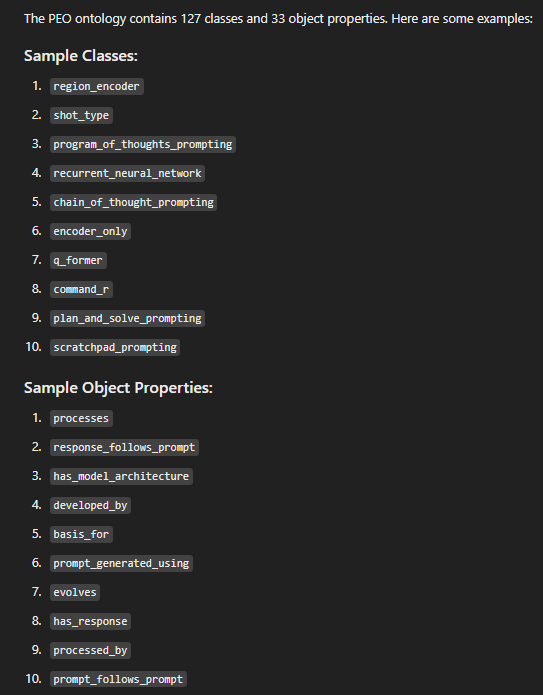
\includegraphics[width=0.85\linewidth]{Figures/fig_36.png}
    \caption{Structure analysis of the ontology}
    \label{fig:enter-label}
\end{figure}
Finally it produces the downloadable RDF file containing the ontology populated by the model.
\begin{figure}[H]
    \centering
    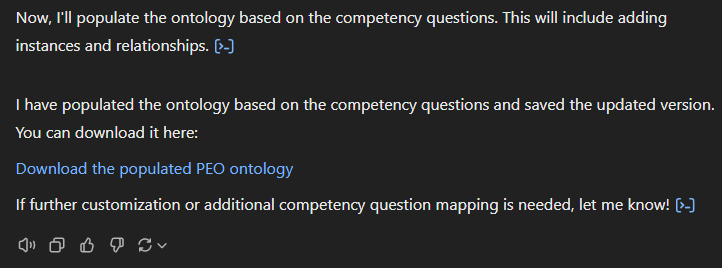
\includegraphics[width=0.9\linewidth]{Figures/fig_37.png}
    \caption{Final LLM output}
    \label{fig:37}
\end{figure}
Fig. \ref{fig:37} shows the final LLM output.
After downloading the RDF file, we open it using the Protegé editor to check the final result.
At a first glance, the obtained result seems rather poor, as four new classes have been created again without considering the classes already present in the ontology:
\begin{itemize}
    \item PromptEngineering
    \item Prompt
    \item PromptingTechnique
    \item Task
\end{itemize}
The class hierarchy is disregarded too as shown in Fig. \ref{fig:38}
\begin{figure}[H]
    \centering
    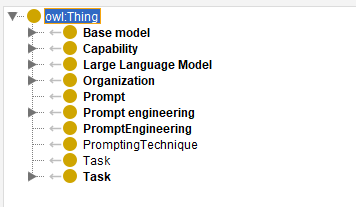
\includegraphics[width=0.9\linewidth]{Figures/fig_38.png}
    \caption{PEO populated automatically}
    \label{fig:38}
\end{figure}
Just two classes have a definition: Prompt and PromptEngineering with no individuals created while the PromptingTechnique class has no defintion and three individuals created:
\begin{itemize}
    \item ChainOfThoughtPrompting
    \item FewShotPrompting
    \item ZeroShotPrompting
\end{itemize}
There is no new instance of chat and all the mechanism defined to link a prompting technique with a chat is completely ignored.
No new object properties or data properties have been created by GPT-4o, just an annotation property called hasDefinition. Any other useful information is not created, the three entities are not linked with any object property and they do not have any data property. Additional prompts would clearly be needed as input for the LLM to improve the result, which is currently poor and adds no useful information compared to the original, manually populated version of the prompt engineering ontology.